\chapter{Entwurfsmuster}

Für \glqq Chess of Duty\grqq{} wurde ein Observer-Pattern eingebaut.

\begin{figure}[h!]
    Commit:  \scriptsize https://github.com/clemens1403/AdvSWE/commit/c04b243f87959c6f80f7d75ccf31cba30af50bd5
\end{figure}

Ein Observer, auf deutsch auch Beobachter genannt, ist ein Entwurfsmuster in der Software-Entwicklung die eine lose Kopplung zwischen Objekten ermöglicht.
Mit Observern können 1:N-Beziehungen hergestellt werden, wobei die Änderung an einem Objekt automatisch an alle abhängigen Objekte weitergegeben werden.
Das Pattern basiert auf zwei Bestandteilen:

\begin{itemize}
    \item Subject: Ist das Element im Code, welches als Beobachtungsgrundlage dient. 
    Das Subjekt enthält eine Liste aller registrierter Observer und stellt Methoden zur Registrierung, Entfernung und Benachrichtigung bereit. 
    Sobald das Subjekt Veränderungen erfährt, werden diese automatisch an alle registrierten Observer übergeben.
    \item Observer: Ein Observer implementiert die vom Subject definierte Schnittstelle, um Benachrichtigungen zu erhalten, um auf die Änderungen  der Subjects reagieren zu können.
\end{itemize}

Damit das Schachspiel nutzbar ist, müssen alle grafischen Elemente regelmäßig gezeichnet werden.
Dabei muss immer der neueste Zustand des Spiels dargestellt werden, welche die Informationen aus der Application-Schicht entnimmt und über die Plugin-Schicht zeichnet. 
Den Zeichner-Klassen müssen Änderungen des aktuellen Spielstandes mitgeteilt werden, sobald sie auftreten.

Im Folgenden wird sowohl der Stand vorher und der Stand nachher genauer beschrieben. 
Für die visuelle Darstellung werden UML-Diagramme verwendet. 
Im Kontext des gesamten Projekts sind die betrachteten Klassen ziemlich umfangreich und weisen eine hohe Anzahl an Attributen und Funktionen.
Um die Diagramme nicht mit unnötiger Komplexität zu überladen, wurde die Darstellung auf die wichtigsten Klassenbestandteile für die Implementierung des Observer-Pattern reduziert. 

\newpage

\section{Vor dem Entwurfsmuster}

Auch ohne die Implementierung des beschriebenen Beobachter-Musters musste für den funktionierenden Programmablauf der aktuellste Spielzustand aus der Spiellogikklasse an die Zeichnerklassen übergeben werden, um die grafische Oberfläche korrekt zu zeigen. 
Processing besitzt eine draw()-Methode, die zur Zeichnung von Grafiken genutzt werden kann. 
In dieser Methode werden die einzelnen Zeichnerklassen koordiniert, sodass alle grafischen Elemente mehrmals die Sekunde gezeichnet werden. 

\begin{minipage}{\linewidth}
    \centering
    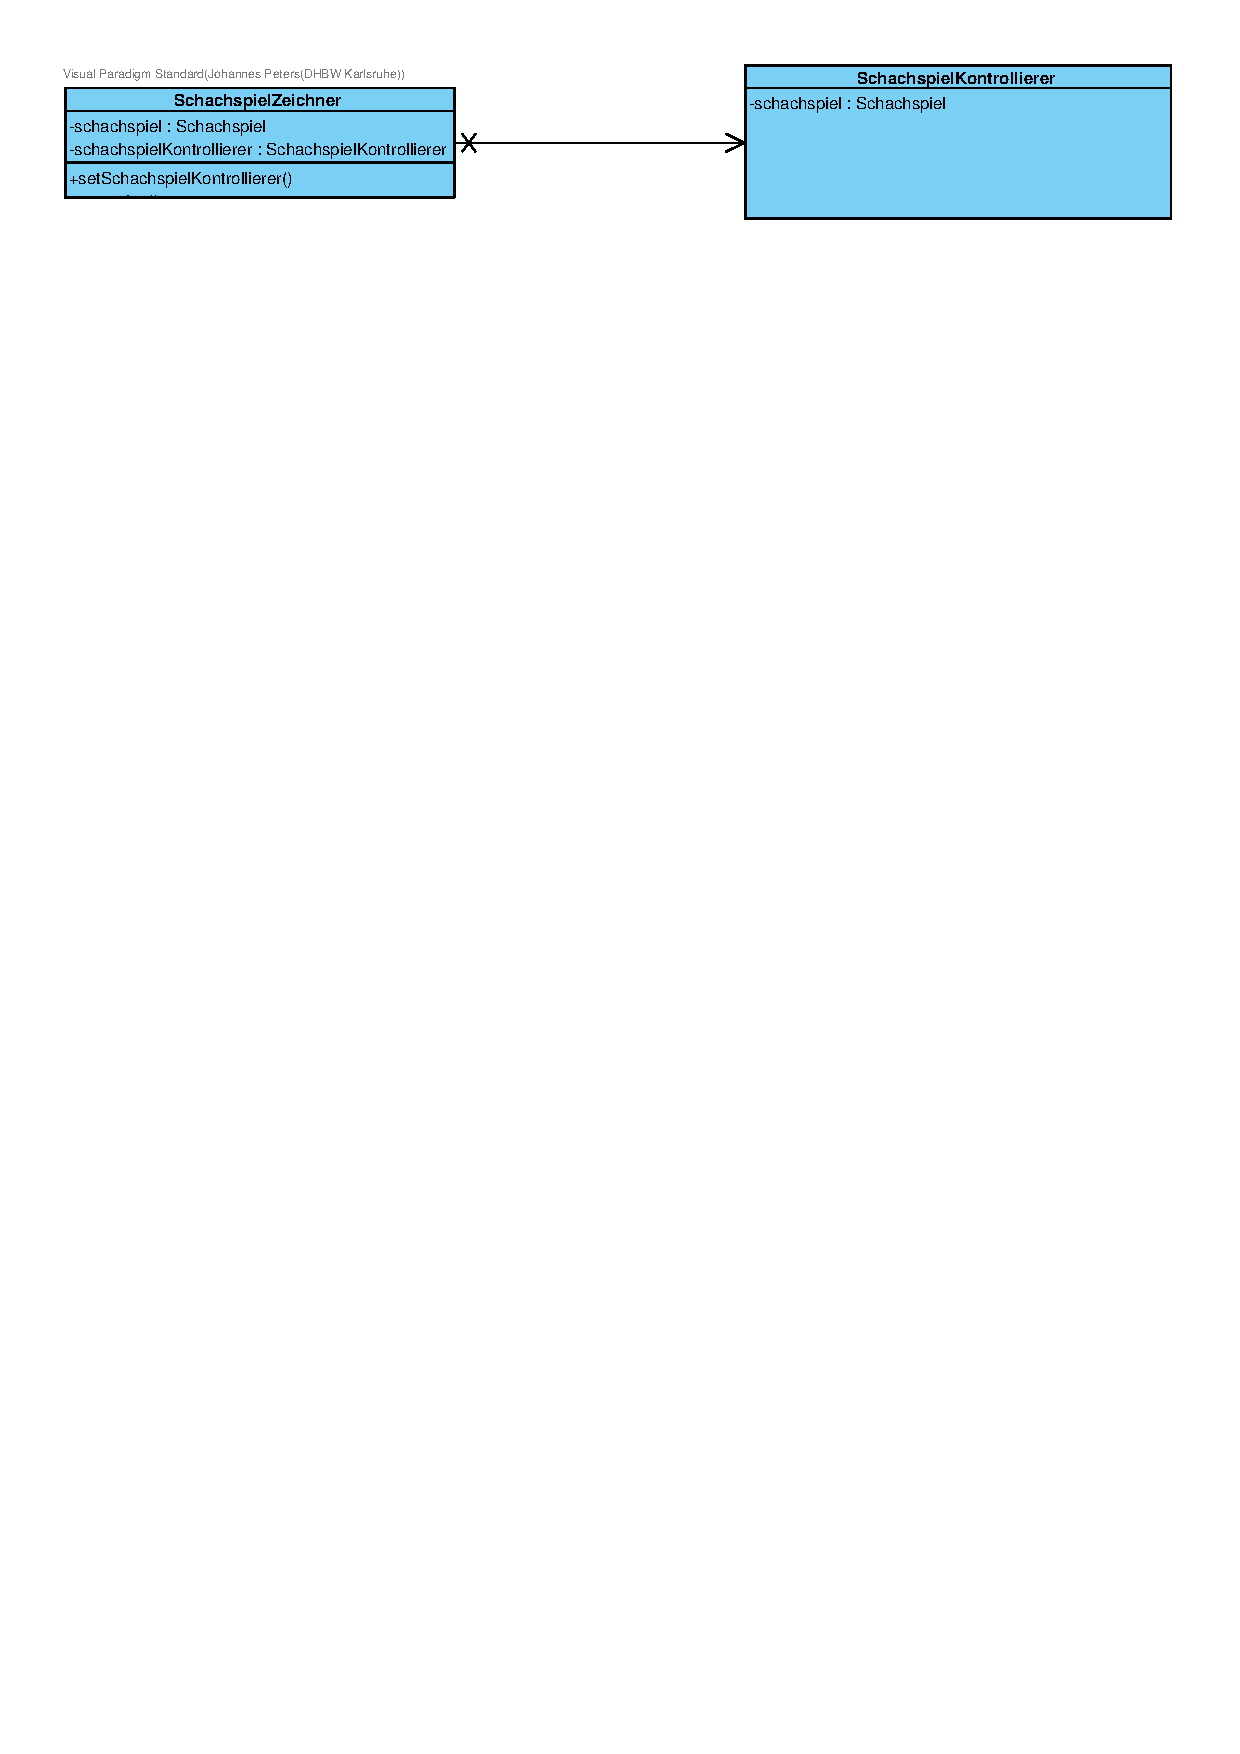
\includegraphics[scale=0.75, trim={0 25cm 0 0}]{Bilder/SWE_ohne_Observer.pdf}
    \captionof{figure}{Programmausschnitt ohne Observer-Pattern}
\end{minipage}

Nach ursprünglicher Implementierung wurde bei jedem Aufruf der draw()-Methode in der Zeichenklasse die Funktion \texttt{setSchachspielKontrollierer} aufgerufen.
Die Methode der Klasse \texttt{SchachspielZeichner} nimmt \texttt{SchachspielKontrollierer} entgegen und setzt diesen als globale Variable in der Zeichnerklasse. 
Da jede übergebene Kontrollierer-Instanz die Variable \texttt{Schachspiel} enthält, kann auch diese Variable lokal in der Zeichnerklasse gesetzt werden, damit auf deren Basis die Grafiken erstellt werden.

\newpage

\section{Mit dem Entwurfsmuster}

Um ein Beobachter-Pattern einzubauen, werden zwei zusätzliche Klassen benötigt, ein Interface für den Beobachter und ein Interface für das Subjekt.
Für den Programmentwurf wurde ein Beobachtermuster für das Attribut Schachspiel erstellt, um alle Änderungen zu registrieren.

Eine Interfaceklasse für einen \texttt{Beobachter} beschreibt die Methode \texttt{aktualisiere()}.
Das Interface für das Subjekt umfasst Methoden zum Registrieren, zum Entkoppeln und zur Benachrichtigung von Beobachtern. 
Diese Methoden müssen bei der Verwendung der Interfaces in verschiedenen Klassen überschrieben werden, um deren Funktion genauer zu beschreiben. 

\begin{minipage}{\linewidth}
    \centering
    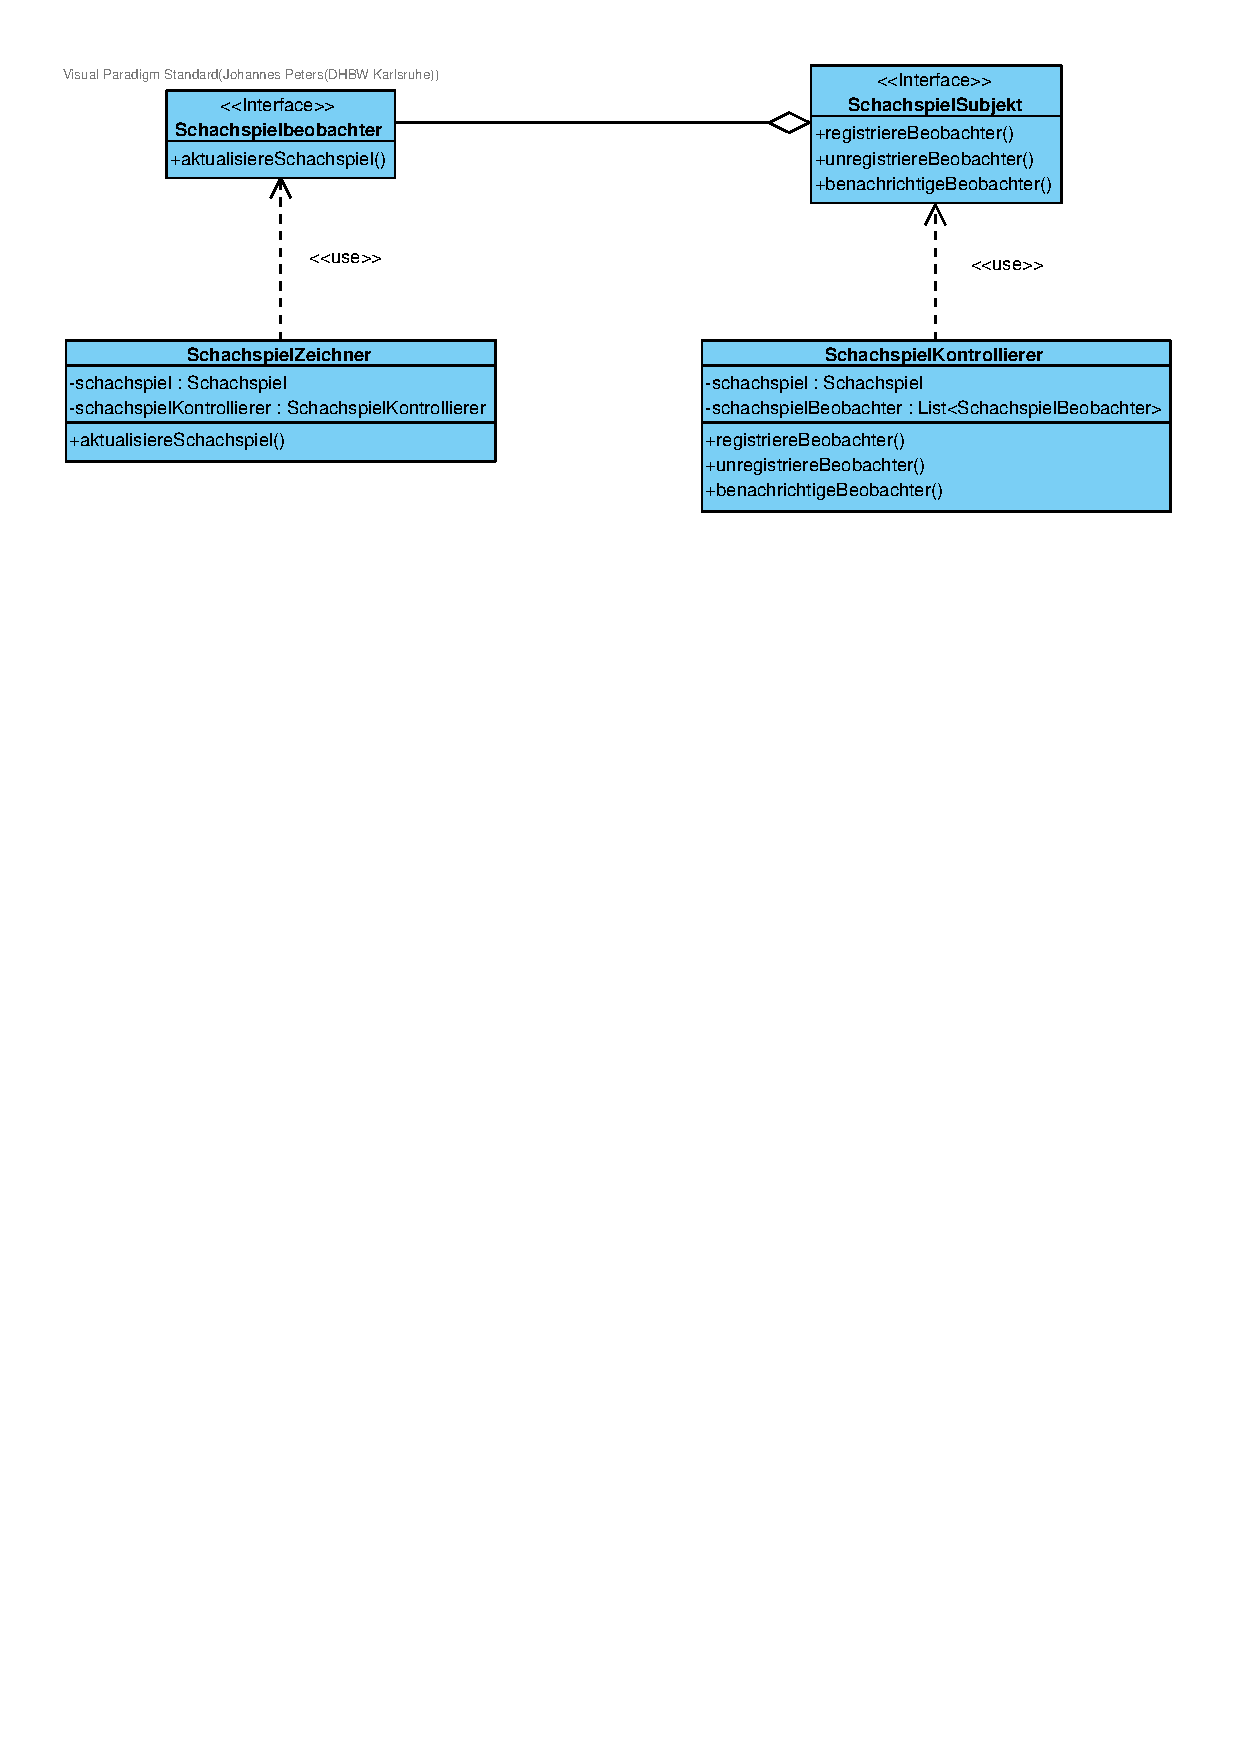
\includegraphics[scale=0.75, trim={0 20cm 0 0}]{Bilder/SWE_mit_Observer.pdf}
    \captionof{figure}{Programmausschnitt mit Observer-Pattern}
\end{minipage}

In der eigenen Implementierung für das Schachprogramm verwendet die Zeichnerklasse \texttt{SchachspielZeichner} das Interface des Beobachters.
Die Spiellogik-steuernde Klasse \texttt{SchachspielKontrollierer} implementiert das Interface für das Subjekt. 
Da beide Klassen jeweils ein Interface verwenden, müssen die in den Interfaces beschriebenen Methoden überschrieben und ausprogrammiert werden. 

Im Kontrollierer wird eine Liste an Beobachtern angelegt.
Die bereits im Interface beschriebenen Methoden \texttt{registriereBeobachter()} und \texttt{unregistriereBeobachter()} verwalten die Beobachter-Instanzen, sofern ein neuer Beobachter hinzugefügt oder ein bestehender Beobachter entfernt werden soll. 
\texttt{benachrichtigeBeobachter()} ist eine Methdoe, bei der durch die Liste an Beobachtern iteriert und für jeden Beobachter die Funktion \texttt{aktualisiereSchachspiel()} aufgerufen wird.

In der Zeichnerklasse wird das Beobachter-Interface verwendet.
Dabei muss die Methode \texttt{aktualisiereSchachspiel()} überschrieben werden. 
Dabei übernimmt diese neue Methode die ursprüngliche Funktion der Methode \texttt{setSchachspielKontrollierer}.
Für die genaue Umsetzung bedeutet es, dass diese neu geschriebene Methode durch den Beobachteraufruf einen neuen Kontrollierer übertragen bekommt, aus welchem die neueste Version von \texttt{schachspiel} entnommen werden kann, nachdem eine Änderung an diesem Attribut auftritt. 

Wenn man die Stände von vorher und nachher betrachtet, könnte man meinen, dass kein wirklicher Mehrwert geschaffen wurde, sondern nur eine höhere Komplexität im Code eingebaut wurde. 
Doch dem ist nicht so. 
Anfänglich wurde bei jedem Zeichenaufruf durch die draw()-Methode von Processing das Attribut \texttt{schachspiel} an die Zeichnerklasse übergeben. 
Das Observer-Pattern verhindert nun, dass mehrmals die Sekunde unnötigerweise das Attribut neu gesetzt wird. 
Mit den eingebauten Beobachter für das Schachspiel-Attribut wird die \texttt{schachspiel} nur dann neu gesetzt, wenn sie explizit vom Subjekt übergeben wird.
Eine Übergabe wird dabei nur dann ausgelöst, wenn sich das Schachspiel-Attribut ändert. 
